\documentclass[
BCOR=5mm,           % Binderkorrektur von 5mm vorsehen
DIV10,              % Seite in X Kästchen einteilen (Siehe Koma-Script Guide)
%DIVcalc,           % Besten DIV Wert berechnen (Siehe Koma-Script Guide)
fontsize=11pt,      % Schriftgröße 11 Punkte
oneside,            % Einseitig
parskip,            % Paragraphen nicht einrücken
headsepline,        % Kopfzeile nach unten durch Linie abgrenzen (scrheadings)
%footbotline,       % Fußzeile nach unten durch Linie abgrenzen (scrheadings)
plainheadsepline,   % Kopfzeile nach unten durch Linie abgrenzen (scrplain)
plainfootbotline,   % Fußzeile nach unten durch Linie abgrenzen (scrplain)
%headtopline,       % Kopfzeile nach oben durch Linie abgrenzen (scrheadings)
footsepline,        % Fußzeile nach oben durch Linie abgrenzen (scrheadings)
plainheadtopline,   % Kopfzeile nach oben durch Linie abgrenzen (scrplain)
plainfootsepline,   % Fußzeile nach oben durch Linie abgrenzen (scrplain)
headexclude,        % Kopfzeile nicht als Teil des Inhalts setzen
footexclude,        % Fußzeile nicht als Teil des Inhalts setzen
%bibtotocnumbered,  % Literaturverzeichnis nummeriert ins Inhaltsverzeichnis aufnehmen
bibtotoc,           % Literaturverzeichnis ins Inhaltsverzeichnis aufnehmen
%liststotocnumbered,% Sonstige Verzeichnise nummeriert ins Inhaltsverzeichnis aufnehmen
liststotoc,         % Sonstige Verzeichnise ins Inhaltsverzeichnis aufnehmen
idxtotocnumbered    % Index nummeriert ins Inhaltsverzeichnis aufnehmen
%idxtotoc           % Index ins Inhaltsverzeichnis aufnehmen
]{scrbook}          % Koma-Script Klasse zum setzen eines Buchs

% Die "Standard-Header" für deutsche Dokumente
\usepackage[latin1]{inputenc}    % ISO-8859-1 bzw. Latin1 als Encoding
\usepackage[T1]{fontenc}         % T1 Schriften verwenden (sieht besser aus)
\usepackage[english]{babel}      % Neue deutsche Rechtschreibung und Übersetzungen

% "Schönere" Schriften einbinden
\usepackage{mathpazo}            % Serifen-Font mit passendem Math-Font
\usepackage[scaled=.95]{helvet}  % Serifenloser Font passend zu mathpazo
\usepackage{courier}             % "Schönerer" Festbreiten-Font

% Koma-Script Paket zum setzen vom Kopf- und Fußzeilen einbinden
\usepackage{scrpage2}
% Seitenstil für normale Seiten auf scrheadings setzen
% Für Kapitelanfang und ähnliches wird scrplain verwendet
\pagestyle{scrheadings}
% Kopf- und Fußzeile löschen
\clearscrheadfoot
% Automarkierungen verwenden \automark[rechts]{links}
% Statt \leftmark und \rightmark kann dann bei
% Koma-Script einfach \headmark verwendet werden
\automark[section]{chapter}
% Kopfzeile für scrplain und scrheadings setzen
% \*head[scrplain]{scrheadings}
%\ihead[Innen]{Innen}
%\chead[Mitte]{Mitte}
\ohead[\sffamily\scshape\bfseries\large\headmark]
{\sffamily\scshape\bfseries\large\headmark}
% Fußzeile für scrplain und scrheadings setzen
% \*foot[scrplain]{scrheadings}
%\ifoot[Innen]{Innen}
%\cfoot[Mitte]{Mitte}
\ofoot[\sffamily\thepage]{\sffamily\thepage}
% Trennlinien für Kopf- und Fußzeile formatieren
% Siehe Optionen der Dokumentklasse
%\setheadtopline{2pt}
\setheadsepline{.4pt}
\setfootsepline{.4pt}
%\setfootbotline{2pt}

% Paket zum Einbinden von Quellcode als Listings
% Hinweis: UTF-8 Encoding führt zu Problemen mit Umlauten
\usepackage{listings}
% Formatierung der Listings
\lstset{
captionpos=b,                % Beschriftung unterhalb (bottom)
numbers=left,                % Zeilennummern links
frame=trbl,                  % Rahmen zeichnen (top, right, bottom, left)
basicstyle=\small\ttfamily,  % Festbreitenschrift verwenden (small)
language=Java                % Sprache auf Java einstellen
}

% Paket für definierte Übersetzungen einbinden
\usepackage[USenglish]{translator}

% Paket für Stichwort- Abkürzungs- und sonstige Verzeichnisse einbinden
\usepackage[
nonumberlist, % Keine Seitenzahlen anzeigen
acronym,      % Abkürzungsverzeichnis erstellen
toc,          % In Inhaltsverzeichnis aufnehmen
%section       % Verzeichniseintrag als Section
]{glossaries}

% Ein eigenes Verzeichnis definieren (Smbolverzeichnis)
% Das Stichwort- und Abkürzungsverzeichnis wird analog vordefiniert
% Siehe makeindex Aufrufe - Hier werden die Dateiendungen festgelegt
\newglossary[slg]{symbolslist}{syi}{syg}{Symbolverzeichnis}

% Den Punkt am Ende der Beschreibung deaktivieren
% \renewcommand*{\glspostdescription}{}

% Stichwort-, Abkürzungs- und Symbolverzeichnis erzeugen
\makeglossaries

% Paket für Wortindex einbinden
\usepackage{makeidx}

% Wortindex erzeugen
\makeindex

% Paket zum generieren von Blindtext
\usepackage{blindtext}

% Paket zum Einbinden von Bildern
\usepackage{graphicx}

%              
% WORKAROUND, damit lstlistoflistings funktioniert:
% Quelle: http://www.komascript.de/node/477
%
\makeatletter
\@ifundefined{float@listhead}{}{%
    \renewcommand*{\lstlistoflistings}{%
        \begingroup
    	    \if@twocolumn
                \@restonecoltrue\onecolumn
            \else
                \@restonecolfalse
            \fi
            \float@listhead{\lstlistlistingname}%
            \setlength{\parskip}{\z@}%
            \setlength{\parindent}{\z@}%
            \setlength{\parfillskip}{\z@ \@plus 1fil}%
            \@starttoc{lol}%
            \if@restonecol\twocolumn\fi
        \endgroup
    }%
}
\makeatother

% My stuff

\usepackage[onehalfspacing]{setspace}
\usepackage{svg}
\usepackage{amsmath}
\usepackage{float}
\usepackage{listings}
\lstset{showstringspaces=false}


\usepackage{hyperref}
\hypersetup{
	breaklinks=true,
	%            colorlinks=true,
	colorlinks=false,
	urlcolor=blue,
	citecolor=blue,
	citebordercolor=0 0 0,
	filebordercolor= 0 0 0,
	urlbordercolor=0 0 0,
	linkbordercolor=0 0 0,
	pdfborder=0 0 0,
	pdfstartview=FitV
}

% Beginn des eigentlichen Dokuments

\begin{document}

% Titelseite (verwendet pagestyle=empty)
\begin{titlepage}
\begin{center}
\includegraphics[scale=2.5]{bilder/he_logo.pdf}\\
\vspace{0.5cm} Department of Computer Engineering\\
\vspace{1.5cm} \Huge Web-Based Deep Learning Algorithms for Classification of Human Cells \\
\vspace{1.5cm} \Large Bachelor Thesis\\\normalsize
\vspace{1.5cm} \Large Christoph Friedrich\\\normalsize
\vspace{0.5cm} Summer Term 2018\\\normalsize
\vfill{}
\begin{tabular}{rl}
First Advisor: & Prof. Dr. J�rgen Koch, University of Applied Sciences Esslingen\\
Second Advisor: & M.Sc. David Dao,  ETH Z�rich\\
\end{tabular}
\end{center}
\end{titlepage}


% Declaration
\chapter*{Declaration}
\thispagestyle{empty}
Ich versichere, dass ich diese Bachelorarbeit selbst�ndig verfasst und nur die angegebenen Quellen und Hilfsmittel verwendet habe.

I assure the single handed composition of this bachelor thesis only supported by declared resources.
\vspace{1cm}
\begin{center}
\begin{tabular}[h]{lp{2cm}p{5.5cm}}
Esslingen, \today &  & \\
\cline{1-1}\cline{3-3}
Place, Date&  & Christoph Friedrich\\
\end{tabular}
\end{center}

% "Frontmatter" beginnen (Formatierung umschalten)
% Platz f�r Inhaltsverzeichnis und anderes
\frontmatter

% Inhaltsverzeichnis ausgeben
\tableofcontents

% Abbildungsverzeichnis ausgeben
\listoffigures
% Tabellenverzeichnis ausgeben
% \listoftables
% Das Listings-Verzeichnis scheint mit manchen Versionen vom Koma-Script
% bzw. des Listings Pakets nicht ohne weiteres zu funktionieren
%\lstlistoflistings

% Definiert die deutschen Eintr�ge im Inhaltsverzeichnis
% Direkt vor \printglossary einbinden
\deftranslation[to=German]{Acronyms}{Abk�rzungsverzeichnis}
\deftranslation[to=German]{Glossary}{Stichwortverzeichnis}

% Die �berschrift f�r den Eintrag mit title= �berschreiben
% Ohne Angabe des type wird type "glossary" verwendet
% Ausser "altlist" existieren einige andere Stile wie z.B. "long"

% Das selbstdefinierte Verzeichnis ausgeben
\printglossary[type=symbolslist, style=long, title=Symbolverzeichnis]
\newpage

% Hauptteil beginnen (Formatierung umschalten)
\mainmatter

%------------------------------------------------------------------
%                      Kapitelstruktur einf�gen
%------------------------------------------------------------------
%\chapter{Motivation}

These days a lot of data is collected to improve the way cars are used or phones are unlocked. Autonomous driving and face recognition are two examples where large data sets are required to improve algorithms and thereby make cars more capable and phones easier to use. 

One of the most interesting areas large collections of data can be
used with significant benefits is in health care. Modern
technologies provide
possibilities beyond anything that could have been 
conceived just a few years back. 
For example, artificial
intelligence enables identifying malignant melanomas by
discriminating them from harmless moles using a standard cellphone camera.

However, a lot of high potential data is still being unused. 
One reason is that computer laymen often don't know how to use the data they already have. \index{computer laymen}
It seems to be a privilege of computer scientists and computer enthusiasts to take advantage of such data and the potential it holds. 

For example, if biologists and doctors had a tool that would 
help them classify and structure their specimen
in an easy way, or even automate such work, it could vastly
increase their productivity and diagnostic capacity.

The objective of this bachelor thesis is to provide a solution to regular
users without any computer science background so they can access the
potential of machine learning in their daily work to assist them
in performing intellectually demanding tasks. The thesis was developed in
the context of biological cell qualification, but can be applied to any
other domain as well.

% Stated a little pathetically: This project wants to help democratizing access to artificial intelligence.
%\chapter{Architecture and Technology}
This chapter is about introducing different software architectures and technologies that are used to build web applications. It is structured as followed. First it shall be explained why web applications offer possibilities desktop application can not. Further a glimpse into JavaScript will be taken. After that a more detailed look will be taken on React and its underlaying software architecture Flux. Further a web framework for managing states called Redux and a JavaScript library for machine learning within the browser, TensorFlow.js will be discussed.

\section{Software application architectures}
Most software applications fall into one of these
categories:

\begin{itemize}
	\item Desktop application
	\item Web application
	\item App for mobile devices
\end{itemize}

There is a clear trend towards web applications as they come
with two significant benefits:

\begin{itemize}
	\item No installation is required by the end user
	\item The runtime environment (web browser) is usually
	      available on all platforms and standardized
\end{itemize}

This trend is reflected by the usage of \gls{JS} as 
the programming language of choice for web applications 
(see Fig. \ref{fig:JSgithub}).
\begin{figure}[ht]
	\centering
	\includegraphics[width=\linewidth]{bilder/grundlagen/jsUsage.png}
	\caption{Github repositories using JavaScript 2014} source:\cite{GitHut}
	\label{fig:JSgithub}
\end{figure}

\section{JavaScript}
Today JavaScript is one of the most used programming languages world wide.
%There are a few big advantages offered by \textbf{\gls{JS}}.\\
% Maybe the biggest advantage is that it comes with the web browser, 
% so everybody can run it by simply typing in an \gls{URL}. This 
% offers great possibilities, since the users don't have to install 
% any software package. The provided application is immediately 
% ready to use once it was loaded.


JavaScript first appeared in 1995. Originally developed at Netscape
 by Brendan Eich under the name of "LiveScript" it had a simple purpose, namely to dynamically manipulate the HTML Document Object Model (DOM) tree in the browser.
 
At about the same time a company called Sun worked on a programming
 language for embedded and mobile devices called Java.   
 As Java became more and more popular,
  Netscape considered it a good marketing move to rename its
  LiveScript to Javacript, even though there was little technological
  similarity between these two languages.
    

Java is a regular, static, and highly typed programming language.
 It runs on a virtual machine and needs to be compiled, whereas the
  single threaded \gls{JS} only runs in a browser and is script
  language. 
  
  Nevertheless they share a C related syntax and some 
  similarities regarding naming conventions. While Java is a true
  object oriented language, JavaScript has incorporated elements
  supporting object oriented programming only over time. \cite{Bewersdorff2018ObjektorientierteProgrammierung}
  
The following analysis shall show why Java Script is in many ways superior for web development. Jeff Attwood the co-founder of the  computer programming question-and-answer website Stack Overflow and Stack Exchange once said "Any application that can be written in \gls{JS}, will eventually be written in JavaScript". \cite{HistoryJS1} \cite{HistoryJS2} \cite{HistoryJS3} \cite{Louis2018Java}

\subsection{JavaScript distributed architectures}

Most modern web designs rely on a three-tier architecture (Fig. 
\ref{fig:TT}). On the server side computation is done and data 
is stored in databases. The client fetches data from the server and 
makes it accessible at the user interface. Often the user is able 
to change data on the client side. \cite{GOLL}

\begin{figure}[H]
	\centering
	\includegraphics[width=0.5\linewidth]{bilder/grundlagen/Three-Tier.png}
	\caption{Three-Tier architecture} source: Reprinted from \cite{GOLL}
	\label{fig:TT}
\end{figure}

For example, to delete or add a user a request is sent to the 
server and a database change is done. For client side it facto 
mandatory to use \gls{JS}, but on server side  a large spectrum of 
languages is available, Java, CSharp, PHP, Ruby these are just the 
most famous one.

Once a user is added on client side, code is needed there in JavaScript. Same action needs to be implemented in a different language on server, 
therefore a second implementation is needed for the same action.
But the JavaScript ecosystem is undergoing rapid growth, with Node.js \gls{JS} is coming to the server and developers are now able to create complete applications in \gls{JS}.

That's big step, distributed systems that can use shared modules. It even affects the job market, front-end developers and back-end developers have been two separated jobs for over decades but now are one. People do not need to learn two languages anymore if they want to do full-stack web development, everything is covered with JavaScript.

\begin{figure}[H]
	\centering
	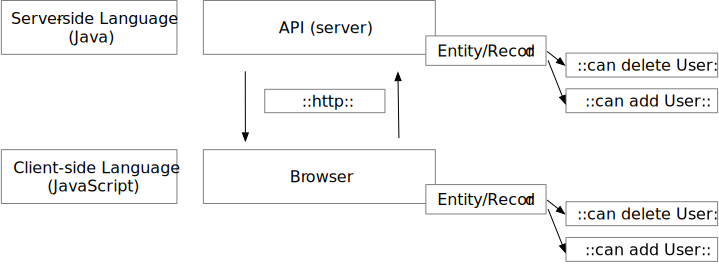
\includegraphics[width=0.8\linewidth]{bilder/grundlagen/Entity1.png}
	\caption{No shared modules} source: Own illustration
	\label{fig:DS1}
\end{figure}

\begin{figure}[H]
	\centering
	\includegraphics[width=0.8\linewidth]{bilder/grundlagen/Entity2.png}
	\caption{With shared modules} source: Own illustration
	\label{fig:DS2}
\end{figure}


\subsection{Multi-Platform support}

Deploying an application for the web browser is only one aspect of modern web development, often a separate implementation is needed for mobile devices or even desktop implementations. Two major operating systems are currently dominating the smart-phone market Android and IOS. 

Both support native App developing but that brings back the problem of having to implement the same functionality twice. Sure smart-phone Apps are different from browser based applications, starting with the touch event and ending up with totally different layouts. 

With JavaScript developers can take advantage of modern frameworks like React Native or Electron, which give the possibility to code in \gls{JS}, the JavaScript is communicating natively with implemented components written in Java on Android, Objective C on iOS, CSharp on Windows via an abstraction called bridge. Everytime \gls{JS} is called it forwards the call to the native code implementation, the response is passed back to the implemented abstraction \gls{JS}. \cite{Purewal2014LearningWeb}

\begin{figure}[H]
	\centering
	\includegraphics[width=0.8\linewidth]{bilder/grundlagen/BridgePattern.png}
	\caption{Bridge pattern} source: Reprinted from \cite{GOLL}
	\label{fig:BP}
\end{figure}


\subsection{Single threading and concurrency}
The single treaded paradigm and non blocking architecture \gls{JS} is bond to, can be considered a weakness. Developing with JavaScript will generate errors and behavior that is perplexing . This section is about analyzing why \gls{JS} is relying on single threading and how it is still possible to add concurrency. \cite{Steyer2014JavaScript}

\gls{JS} was developed to manipulate the DOM, the DOM is a limited resource. Executing two pieces of code, asynchronously changing the same part of DOM would not be good. Given this single purpose it was decided to make JavaScript single threaded.

Actions that do not change the DOM should be able to run asynchronously. That makes sense, since fetching data from the server or reading a large list of files can take a lot of time and would block the browser, buttons would not be clickable anymore and any rendering would stop. 

How is it possible that JavaScript offers the opportunity to run code concurrently, even though it is single threaded? The following example how multi-threading is implemented in JavaScript.

Every time a function in \gls{JS} is called, it is put on the call stack. The result of that function is popped out from stack. The functions on stack are executed synchronously one after another.

\begin{figure}[H]
	\centering
	\includegraphics[width=0.8\linewidth]{bilder/grundlagen/CallStack.png}
	\caption{Call Stack} source: Own illustration
	\label{fig:CS}
\end{figure}

To execute code concurrently JavaScript needs to call the Web API, provided by the browser. The web browser is written in C++, so it fully supports multi-threading.

The Web API is called with a function that needs to be executed and a callback.
The callback tells what to do after the asynchronous function finished executing. It is mandatory to provide a callback with each asynchronous function.

Once the thread finished executing it passes the callback to as so called Callback Que. The Callback Que is a simple list with all callbacks that need to be executed. 

Further an event loop is responsible for checking if current stack is empty, if that's the case, the callback is put on stack and executed synchronously. The decoupling of the caller from the response allows for JavaScript to do other things while waiting for asynchronous operations to complete and their callbacks to fire. 

\begin{figure}[H]
	\centering
	\includegraphics[width=0.8\linewidth]{bilder/grundlagen/Concurrency.png}
	\caption{Concurrency in JavaScript} source: Own illustration
	\label{fig:CC}
\end{figure}

\subsection{Functional programming paradigm}
There is no need to use functional programming in JavaScript, since this is more a philosophy question and definitely nothing somebody needs to do when programming in JavaScript.Other ways of coding, like object oriented programming, are supported in JavaScript as well. This section shall explain what functional programming is and how it is implemented in JavaScript. No global variables or states are used in functional programming, the output of a function only depends on the input arguments.

\begin{figure}[H]
	\centering
	\includegraphics[width=0.8\linewidth]{bilder/grundlagen/fp.png}
	\caption{Imperative and functional programming} source: Own illustration
	\label{fig:FP}
\end{figure}

Another concept is the use of high-order functions. Giving the possibility to use functions as inputs and outputs. 


\begin{figure}[H]
	\centering
	\includegraphics[width=0.5\linewidth]{bilder/grundlagen/fp1.png}
	\caption{High-order functions} source: Own illustration
	\label{fig:HF}
\end{figure}

Data mutation shall be avoided.

\begin{figure}[H]
	\centering
	\includegraphics[width=0.8\linewidth]{bilder/grundlagen/fp2.png}
	\caption{Data mutation} source: Own illustration
	\label{fig:DM}
\end{figure}

\newpage

\section{Software patterns for web-development}

\subsection{Classic MVC model}
For decades it was best practice to use the Model View Controller software architecture. The model stores the data presented in a view, in simple systems the model may contain business logic.

The model shall be independent of views and controllers. In case the model changes the controller may inform the views (passive Model). With an alternative active model implementation, the model informs the views. One model can have multiple views.
 
The view serves to present model data to user, there can be many views on the same model data. All views are updated in case of a model data change. A view may furthermore present interactive elements like buttons. 
 
Interaction with these elements creates events that usually are handled by the controller. The controller controls the model and view state, based on user input. It transforms events caused by user action into method calls of the model, the controller furthermore controls the state of view, for example activate or deactivate buttons.


\begin{figure}[H]
	\centering
	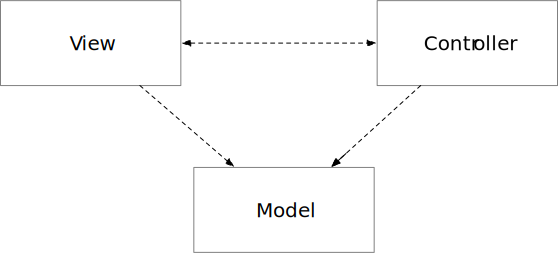
\includegraphics[width=0.8\linewidth]{bilder/grundlagen/MVC.png}
	\caption{MVC  software architecture} source: Reprinted from \cite{GOLL}
	\label{fig:MVC}
\end{figure}


The so called separation of concerns makes it easier to split work and, due to that it makes it easier to maintain code. But it also comes with an increased complex setup process. Changes for example in the model or the controller affect the whole entity. The bidirectional communication in the MVC structure makes it hard to debug, changing one entity  causes a cascading effect across the codebase.

React tries to get rid of that by introducing a different architecture called Flux. The following section shall explain how Flux is different from the MVC pattern.

\subsection{Flux}

\subsubsection{Structure and data flow}

In Flux data flows in a single direction, the unidirectional data flow is central to Flux. Dispatcher, stores and views are independent nodes with different inputs and outputs. The actions simply consist of objects with the new data.


\begin{figure}[H]
	\centering
	\includegraphics[width=0.8\linewidth]{bilder/grundlagen/UniDirection.png}
	\caption{Flux software architecture} source: Reprinted from \cite{Flux}
	\label{fig:FLUX}
\end{figure}

The dispatcher takes care of handling all actions and forwarding it to the right store. The store holds the data and actions to change this data. Once data was changed the store alerts all views that are affected by this data change, causing a re-rendering.

It is also possible that a view generates an action, this happens mainly through user interaction. This action is also passed to the dispatcher. 


\begin{figure}[H]
	\centering
	\includegraphics[width=0.8\linewidth]{bilder/grundlagen/uniDirection2.png}
	\caption{Flux With View Action} source: Reprinted from \cite{Flux}
	\label{fig:FA}
\end{figure}

\subsubsection{Dispatchers}
Dispatchers can be considered as a central hub that is managing all data flows in a Flux application.

The only way to change data, is through actions the dispatcher is providing.
A dispatcher has no real intelligence of its own, it only provides a simple mechanism to distribute action over several stores.

This becomes more important when big applications shall be built. The dispatcher then handles dependencies between different stores, he takes care of updating the different stores in a specific order.

\subsubsection{Stores}
Stores contain the application's logic and states. This role can be considered somehow similar to a model in the traditional MVC, the difference is that stores manage the data of many objects and not a single record of data like ORM models do. They manage the application state for a whole domain. 

For example Facebook's Lookback Video Editor utilized a TimeStore that kept track of the playback time position and the playback state. On the other hand, the same application's ImageStore kept track of a collection of images.

\subsubsection{Views and conroller-views}

In React all views are composable and freely re-renderable. at the top of each view, the highest in hierarchy, there is a view that listens to events that are sent by the store. It is called a controller-view. 

The controller-view fetches the data from store and passes it down to all descendants, causing a re-rendering. Often the entire state of a store is passed down a chain of views allowing each descendant to take what he needs.

\subsubsection{Actions}
As already mentioned action change the store . Each action has payload with new data, every time an action occurs a dispatch is triggered to the stores. User-interaction is not the only of actions, it can also come from other places like the server.


\subsubsection{Conclusion}
The Flux architecture is improving data consistency. The unidirectional data flow makes it much easier to debug. Since one can always follow easily the flow of actions. Furthermore with having the state and all the logic that is updatitng the state at one place it is also possible to do more meaningful unit tests.

\section{React and Flux}

Another key technology used in this project, is React. React is a JavaScript library for developing user interfaces. 

Back in 2011, Facebook noticed that it was getting hard to maintain their Application and to run it flawlessly, because of the growing number of features. Many people were hired and the team size expanded dramatically. With the growing team size it took longer to publish urgent updates, too many people were involved and concerns could not be separated in a satisfying manner.

A Facebook engineer called Jordan Walke decided to change that, in the same year he created FlaxJs, first prototype of React. Jordan was allowed to keep on working and created React (2012). 

A short time later Instagram was bought by Facebook and both companies agreed on using React as the new core technology for User Experience. Further they agreed on making React publicly available. 

In early 2013 at JS ConfUS, React became an open source project. Facebook CEO Mark Zuckerberg, speaking on the this conference said  "Our biggest mistake was betting too much on HTML5" and promised to provide better experiences with React.

Currently React is getting more and more popular. A trend analysis, by Google shows that React is the leading modern User Experience JavaScript framework.

\begin{figure}[H]
	\centering
	\includegraphics[scale=0.4]{bilder/grundlagen/ReactDownloads.png}
	\caption{Downloaded npm packages} source: \cite{NPM}
	\label{fig:JS}
\end{figure}

This section is about analyzing how React is implementing the Flux Software Architecture. React depends on encapsulated components that manage their own state. An application consists of nested components, somehow similar to the tree structure of a HTML DOM.

Components are written in JavaScript, so data can easily passed through the Application. Everything that needs to be rendered is still written in HTML and parsed by React. Each component has its own controllers, there is no more discrimination between what is shown in the Browser and business logic.

There are no separated HTML and JavaScript files, only JavaScript. Every component is fully standalone and testable by its own. This makes React scalable and easy to test. There are no cascading dependencies. Every time the state of a component changes, the render function is called and the HTML is re-rendered with the changed data. Components can be nested, e.g. a board game that consists of squares.

\lstinputlisting{code/grundlagen/Component.js}


Each of that squares is a component and part of the whole board game application. There shall bee a value assigned to the squares, values are passed through the prop value.

\lstinputlisting{code/grundlagen/ComponentWithProps.js}


\begin{figure}[H]
	\centering
	\includegraphics[width=0.3\linewidth]{bilder/grundlagen/GameGrid.png}
	\caption{Grid with numbers} source: Own illustration
	\label{fig:RL}
\end{figure}

Now when clicked on a square, this square shall show the 'X'. The value can now be considered a local state, it is definitely a private part of the square. First an initial state needs to be added.

\lstinputlisting{code/grundlagen/ComponentWithState.js}

If this.setState is called, an update is scheduled by React and the value is merged in the correct component state. Furthermore the component and all of its descendants are re-rendered. If a Square was clicked it would now show a 'X' in the grid.

\subsection{Lifting state up}
Often data needs to be aggregated from multiple child components. Then it makes sense to lift all states up to a top-level component. The parent component then passes down the individual states for the child components.

E.g. in a Tic Tac Toe game, to determine who has won, the value of all squares components would need to be checked. That is technically doable, but a better approach is to save all states in the parent component and the parent component can simply check one array, in order to determine who has won. 

The Square component is no longer keeping its own state, it receives the value from its parent Board. It informs the parent when it was clicked. These components are called controlled components. 

\begin{figure}[H]
	\centering
	\includegraphics[width=0.8\linewidth]{bilder/grundlagen/topLevelComponent.png}
	\caption{Top-Level Comonent} source: Own illustration
	\label{fig:RL}
\end{figure}


\subsection{Action- and dataflow}
Taking the last examples it is clear that that is only passed in one way, from the top-level component to a child component. Another key principle is that actions are only passed up. For example if a nested component B is clicked or is triggered on a different event some state B shall be changed in the top-level component. That is possible because all functions that change the data in top-level component can be passed down to nested components via the props variable.

\begin{figure}[H]
	\centering
	\includegraphics[width=0.8\linewidth]{bilder/grundlagen/dataFlow.png}
	\caption{Action- and dataflow} source: Own illustration
	\label{fig:RL}
\end{figure}


\subsection{High-Order components}
As already knwon from the JavaScript introduction chapter
a high-level function takes another function as an argument. Similar to that a High-Order Component is simply a high-order function that takes a stateless component and returns the changed component. This is very practical since it gives the possibilty to give them extra functionality or to even change the wrapped component. 

\lstinputlisting{code/grundlagen/hoc1.js}


\lstinputlisting{code/grundlagen/hoc2.js}



\subsection{Virtual DOM}

Manipulating the DOM is the main thing modern, interactive web applications do. Unfortunately it is a lot slower than running JavaScript. The HTML DOM is always tree structured, which makes it easy to traverse through it, but it also offers poor performance.

Additionally some modern frameworks update the DOM more often than it needs to be updated. For example changing one item in a list of ten items would lead to re-rendering all ten items. React is addressing this problem by introducing a virtual DOM.

The Virtual DOM is an exact representation of the HTML DOM with JavaScript. Once states have changed the virtual DOM is updated first, then the previous Virtual DOM is compared to the current Virtual DOM. Only what is different will be updated in the HTML DOM.

\begin{figure}[H]
	\centering
	\includegraphics[width=0.8\linewidth]{bilder/grundlagen/VirtualDom.png}
	\caption{Virtual DOM comparison} source: Own illustration
	\label{fig:COMPONENT}
\end{figure}


\subsubsection{Conclusion}
React is a relatively new framework with a new underlaying software architecture for user interfaces. This architecture leads to less files and more encapsulation. Therefore it scales better than classic MVC, when having more views on the same data. Due to the virtual DOM React is really performant when updating the DOM.


\subsection{Redux}
Redux is a predictable state container for JavaScript apps. It makes applications more consistent, by organizing all satates in the app. Redux evolves the ideas of the Flux software architecture.
 
The gist of Redux is that all states are kept as an object tree,in a single store. It is only possible to change this object tree by emitting an action, this action is an object describing what happened. To specify how these actions change the state tree, pure reducers are written.

The only difference to Flux is that Redux does not have a Dispatcher or support many stores. There is just a single store with a single root reducer. In bigger applications the root reducer can be split into smaller reducers, each operating independently on the different parts of the state tree.

Redux adds a lot of overhead to an application, a lot of more files and code are created. Considering that Redux should only be used if the following points are true. 

\begin{itemize}
\item Reasonable amounts if data is changing over time
\item A single source of truth is needed
\item Keeping all of the states in a top-level component is no longer sufficient.
\end{itemize}

It should further be mentioned that Redux destroys a key principle of React, by giving the possibility to access the state from all components in an application directly. It is no longer obvious what data is used in which component. The following illustration shall undermine this thesis.

\begin{figure}[H]
	\centering
	\includegraphics[width=0.8\linewidth]{bilder/grundlagen/reduxStore.png}
	\caption{Redux store} source: Own illustration
	\label{fig:COMPONENT}
\end{figure}

\section{TensorFlow.js}
TensforFlow.js is an open source JavaScript library for training and deploying neural networks in the browser and on Node.js. First introduced in spring 2018 it already provides intuitive APIs to build and train models from scratch in the browser. Existing models can be loaded and re-trained, also normal TensorFlow models can be imported and used. The WebGl-accelerated implementation makes it possible to train and predict in a reasonable time. There are a few core concepts of TensorFlow.js, the following subsection will go more into detail.

\subsection{Core Concepts}

In order to train neural networks with images or other data, this data needs to be shaped into numerical arrays. These numerical arrays are called Tensors, a Tensor has a shape attribute that defines the Tensor's dimension. Tensors are immutable, the values of a Tensor can not be changed.

\lstinputlisting{code/grundlagen/tensor.js}

Variables are initialized with a tensor of values. Unlike Tensors, however, their values are mutable.

\lstinputlisting{code/grundlagen/variables.js}

Operations are performed on tensors. TensoFlow.js provides a wide variety of algorithms that can be performed on tensors. This operations do not change the tensor, instead the return new tensors.

\lstinputlisting{code/grundlagen/operations.js}

In TensorFlow.js models are nothing different than a function that takes an input and produces an output. TensorFLow.js provides a high-lovel API called tf.model to construct a model with layers.

\lstinputlisting{code/grundlagen/model.js}

\subsection{Performance}
Even though TensorFlow.js can access the local GPU (Graphics Processing Unit) it is 1.5-2 times slower than TensorFlow distributions written in Python or C++. 
Small models train faster in the browser, however large models train up to 10-15 times slower in the browser compared to TensorFlow written in Python.

\subsection{Conclusion}
TensorFLow.js makes constructing neural networks, training and predicting very easy. The GPU support, makes it running relatively fast, however yet it is not as performant as TensorFlow distributions written in C++ or Python. In a nutshell, TensorFlow.ja has a serious potential, instead of calling a server backend for training and predicting. No data needs to be uploaded, everything can be done on client side. Models can be simply loaded over a CDN (Content Delivery Network).

%\chapter{Deep Learning}

Deep learning is a class of neural network optimization methods for networks that have
 a significant number of hidden layers between their input and output layer.
  Compared to learning algorithms of more simple network structures, the methods of 
  deep learning offer a stable learning success even in the presence of numerous hidden layers.

Deep learning has been successfully applied to object detection in computer vision, in natural language processing,
 and speech recognition. In this chapter we will explain how such artificial neural networks 
 function by looking at feed-forward network as an example. 

\section{Feed-forward neural networks}

A feed-forward network comprises one input layer, H hidden layers and one output layer.
Each layer consists of a number of elements called "neurons". Each neuron of any given layer is 
fully connected to each neuron
of the previous layer. Mathematically, a neural network is represented by a combination of 
matrix multiplication and
activation functions. An activation function determines when a neuron fires.
It usually is nonlinear. The nonlinear characteristic of the activation function is 
what enables the network to learn. Each neuron in a hidden layer can be described by equations \ref{eq:1} and  \ref{eq:2}

\begin{equation} \label{eq:1}
	y_{j} = f(z_{j})
\end{equation}

\begin{equation} \label{eq:2}
z_{j} = \sum w_{ij}*x_{i} + b_{j}
\end{equation}

\begin{figure}[H]
	\centering
	\includegraphics[width=1.0\linewidth]{bilder/grundlagen/fast-forward.png}
	\caption{Schematic view of a  simple two layer fully connected neural network (FCN)}
	\label{fig:FCN}
\end{figure}

The outputs of the preceding layer are each weighted with a weight \(w_{ij}\) before they are accumulated.
The resulting sum is shifted by adding a bias \(b_{j}\) to generate the input \(z_{j}\) for the 
activation function \( f(\cdot) \).
The output of the activation function \(y_{j}\) is then taken as the input for the next 
hidden layer or output layer.
 
 Any continuous functions can be used as activation functions of a neural network. 
 Most common activation functions are sigmoid,  \(f(z) = \dfrac{1}{e^{-z}}\), 
 the hyperbolic tangent, \(f(z) = \frac{exp(z)-exp(-z)}{exp(z)+exp(-z)}\) or the 
 rectifier linear unit (ReLu) \(f(z) = max(0; z)\). ReLu will be used for all future examples.


\begin{figure}[H]
	\centering
	\includegraphics[width=0.8\linewidth]{bilder/grundlagen/sigmoid.png}
	\caption{Sigmoid And ReLu activation function (from\cite{Sigmoid})}
	\label{fig:Sigmoid}
\end{figure}


\subsection{Backpropagation}

Training a neural network means iteratively applying a forward pass followed by an error backpropagation.
During the forward pass the outputs for each neuron are calculated based on its inputs.
The resulting outputs \(y_{out}\) are then compared with the correct answer via a cost function  \(E\).
A common cost function for example is squared error loss (see equation \ref{eq:3}):
 
\begin{equation} \label{eq:3}
	E=\sum\dfrac{1}{2} (target-y_{out}^2) 
\end{equation}

Based on the output of \(E\) it is now possible to check how weights need to be 
adjusted in order to minimize the error.
Applying the chain rule we get equation \ref{eq:4}. 

\begin{equation} \label{eq:4}
	\frac{\partial z}{\partial x} = \frac{\partial z}{\partial y} \frac{\partial y}{\partial x}
\end{equation}

Considering the error  \(E\) we get equation \ref{eq:5}

\begin{equation}  \label{eq:5}
\Delta_{W}E =
\frac{\partial E}{\partial W_{l}} =
\frac{\partial E}{\partial y_{out}}
\frac{\partial y_{out}}{\partial z_{out}}
\frac{\partial z_{out}}{\partial y_{n-1}}
\frac{\partial y_{n-1}}{\partial z_{n-1}}
\end{equation}

Using the calculated gradient $\Delta_{W}E(y_{out})$  it is now possible 
to determine the next weight matrix update using a gradient descent (equation \ref{eq: 6}):

\begin{equation} \label{eq:6}
W_{l}^{t+1}=
W_{l}^{t}-\eta\Delta_{W_{l}^{t}}E(y_{yout)}
\end{equation}

where \(W^{t}\), \(W^{t+1}\) are the current and the updated weight matrices, respectively,
and  \(\eta\) is the learning rate.

\subsection{Weight update}
Calculating the gradient for a complete dataset can take a lot of computation time.
To reduce the amount of computation required
mini-batches can be used to calculate the gradient only based on a few sampled data points. 
Using this analytic gradient a parameter update is performed. There are several ways to perform this update,
the most common one being the stochastic gradient descent (SGD).
In this algorithm, parameters are simply changed along the negative gradient 
direction in order to minimize the error.


\subsection{Initialization}
A neural network needs its weights initialized before it can be trained.
Random initialization is the most common way to create the initial weights.

\subsection{Batch normalization}
To avoid numerical problems due to extreme values the input data is 
normalized (see equation \ref{eq:7}).

\begin{equation}\label{eq:7}
	x \Rightarrow \hat{x} = \dfrac{x-\mu}{\sigma} \Rightarrow x_{norm} = \gamma \hat{x} + \beta
\end{equation}

\(\mu\) and \(\sigma\) are the mean and the  standard deviation of the dataset, respectively. 
\(\gamma\)\ and \(\sigma\) scale and shift the parameters. Batch normalization accelerates 
training time and makes a deep neural network less sensitive to initialization issues.

\section{Classification}
A common task for neural networks is the classification of images, or more general the classification of data into a specific category. The best performing neural network architectures for classifying images are 
convolutional neural networks (CNN). 
All convolutional neural networks consist of convolutional layers followed by pooling 
layers and some fully connected layers.

\subsection{Convolutional layer}
In a convolutional layer several kernels are applied to extract spacial related features. Each output from the the convolutional layer is called a feature-map. Each feature-map was created by a different convolutional kernel of the layer. 

\begin{figure}[H]
	\centering
	\includegraphics[width=\linewidth]{bilder/grundlagen/convolution.png}
	\caption{Schematic view of a Convolutional Neural Network (CNN) (from \cite{Dao})}
	\label{fig:CNN}
\end{figure}

\subsection{Pooling layer}
After features have been extracted into feature maps,  the pooling layer reduces the 
size of the feature maps and makes them computationally  tractable. A simple implementation 
of a pooling layer is the max-pooling layer, which uses a sliding windows over the input and 
selects the maximum of each window.

\begin{figure}[H]
	\centering
	\includegraphics[width=\linewidth]{bilder/grundlagen/pooling.png}
	\caption{Pooling layer (from\cite{Dao})}
	\label{fig:Pooling}
\end{figure}

\subsection{Data augmentation}
Convolutional neural networks need a lot of data to generate satisfactory output. \index{data augmentation}
If not enough data can be provided the data can be artificially augmented by using different approaches.
images can be turned or flipped, cropped, blurred or even resized. This makes it 
possible to generate a lot of data which can be used to further improve training.

\begin{figure}[H]
	\centering
	\includegraphics[width=\linewidth]{bilder/deep_learning/data_aug_basic.png}
	\caption{Data augmentation(from  \cite{Ratner2017})}
	\label{fig:COMPONENT}
\end{figure}


%\chapter{Image Based Profiling}

Modern fluorescence microscopy combined with high throughput biotechnology, automatically quantifying biological properties in images, is now widespread. They provides new insights into human cells and are powerful technologies for studying cell biology. 
Using this technology more than more than 
one hundred thousand  images can be produced per day.
This makes automated image analysis a necessity. 
Image-based profiling aims at getting as much data 
as possible from a biological sample and to encoding
it in a proper way. Image-based profiling experiments capture a wide range of data
from biological samples without prior knowledge
of the existence of any markers.
Data mining and machine learning techniques can then be applied to identify patterns \cite{Jones} \cite{Scheeder2018}.

\subsection{Drug discovery}

One important application of image-based profiling is identifying biological mechanisms of actions (MOA),
for example checking damage of DNA replications due to chemical perturbations.
When developing new drugs and making predictions about unknown
chemical compounds it is important to know what chemical compounds cause which biological mechanisms of action.
Morphological profiles can predict these MOAs for chemical compounds.

\subsection{Typical workflow}

There are two approaches in image-based phenotyping of perturbations. 
It should be considered that they are different.
The first approach is called phenotypic screening. 
Phenotypic screening uses pre-defined, specific phenotypes which are compared 
with the specimen in order to identify drugs or drug targets that might have affected 
them.

The second method is called profiling of perturbations. 
Here a computer is trained with a large set of samples, both
affected by perturbations and unaffected ones.
Once trained the computer can analyze new specimen 
and for perturbed ones identify the drugs or drug targets that have affected them.
This approach doesn't require the specification of any features such as cell size, intensity, shape, or texture.
It furthermore permits how any specimen would look if it was affected by a specific perturbation.


\begin{figure}[H]
	\centering
	\includegraphics[width=0.8\linewidth]{bilder/cells/hcu.png}
	\caption{Typical workflow of image-based small molecule experiments (from \cite{Scheeder2018})}
	\label{fig:Workflow}
\end{figure}

Fig. \ref{fig:Workflow} illustrates a typical workflow of image-based small molecule experiments. First cells need to be attached to plates. In a second step cells are perturbed. Then after staining the cells, images are taken using automated microscopes. At the end either screening approaches (A) or (B) profiling approaches can be used to classify perturbed cells.

\subsubsection{Segmentation}

Small molecule profiling is based on staining subcellular structures (Fig. \ref{fig:ig:Segmentation}).
An accurate segmentation of cells can be achieved by in intensity-based thresholding and other approaches. A number of computational applications for segmentation-free analysis in image-based profiling have been developed, the most famous one being the Cell Profiler \cite{CellProfiler}.


\begin{figure}[H]
	\centering
	\includegraphics[width=0.8\linewidth]{bilder/cells/segmentation.png}
	\caption{Segmentation (from \cite{Pau})}
	\label{fig:Segmentation}
\end{figure}


\subsubsection{Classification}


A typical objective for profiling experiments is the classification of compounds that cells have been perturbed with. 
Common classifiers are random forests and deep neural networks that are employed to achieve higher 
accuracy in predicting biological MOAs.


\begin{figure}[H]
	\centering
	\includegraphics[width=0.8\linewidth]{bilder/cells/classification.png}
	\caption{Classification  (from \cite{Pau})}
	\label{fig:Classification}
\end{figure}





%\chapter{Related work}
This chapter is about presenting CellProfiler Analyst (CPA), a first generation tool for interactive 
data exploration and classification of large biological image sets. 
It was first introduced in 2016 at the Broad Institute of MIT and Harvard. 
The following section gives an overview of CPA's main functionality and an exploration of its key features, 
the classifier and image gallery. 

This project is highly influenced by CPA and basically aims to improve it and make it accessible
to anybody without having to install any software. CPA is free and open source, 
available at \href{http://www.cellprofiler.org}{http://www.cellprofiler.org} and from GitHub under a 
BSD-3 license. It is available as a packaged application for
Mac OS X and Microsoft Windows and can be compiled for Linux.

\subsection{CellProfiler Analyst}
CPA is a GUI based tool. It provides features for data exploration and classification via 
its user interface. There are only a few comparable tools for this purpose, the most prominent being  
Ilastik, CellCognition and WND-CHARM.

All these tools lack a suitable companion visualization tool capable of handling large datasets. 
Furthermore they do not provide selectable classifier algorithms. Another big benefit CPA has compared 
to all other existing tools that it incorporates an interactive object classification and image viewing feature.

\begin{figure}[H]
	\centering
	\includegraphics[width=1.0\linewidth]{bilder/related_work/cpa_main_view.png}
	\caption{CPA main view, different views are selectable  (from \cite{Jones2008})}
	\label{fig:CPA}
\end{figure}

\subsection{Classifier}
The Cell Profiler Analyst Classifier makes it possible to create categories and to classify cells.
 After fetching images from a predefined dataset it is possible to classify images 
 by simply drag and dropping them on a category. Multi-select features are also implemented
  and enable to drag and drop multiple images at the same time. 
  
  Further it is possible to add an unlimited amount of categories by clicking the "add category" button. 
  After annotation is done the algorithms can be trained. Once training is done more images can be 
  fetched and then be automatically annotated by clicking the "evaluate" button. 
  
  If results do not suffice further images can be annotated to train the algorithm. 
  Different algorithms can be used to classify the uncategorized images, such as 
  RandomForest Classifier and AdaBoost Classifier.

\begin{figure}[H]
	\centering
	\includegraphics[width=1.0\linewidth]{bilder/related_work/classifier.png}
	\caption{CPA classifier view (from \cite{Jones2008})}
	\label{fig:Classifier}
\end{figure}


\subsection{Visualization}


In order to explore a dataset and to predict and validate a result, a good visualization is needed. 
CPA offers different ways of displaying data and results. 

One simple visualization possibility is the Image Gallery where images from the dataset can be selected and 
displayed in their original size. Filters can be applied to only select images with experiment specific meta data. 
There are many more ways to display and explore data in CPA.

\begin{figure}[H]
	\centering
	\includegraphics[width=1.0\linewidth]{bilder/related_work/visualization.png}
	\caption{CPA Main View Different Views Are Selectable (from \cite{Jones2008})}
	\label{fig:RL}
\end{figure}


\subsection{Downsides of CPA}
Getting CPA to run on a computer requires installation first. This installation is
not trivial as the system requires a MySQL database system to work.

Furthermore, the powerful user interface makes the system complex and difficult to use. This can 
scare off potential users.






\chapter{CYTO AI}

CYTO AI is the first fully web-based image labeling and classifying tool publicly available. Based on the JavaScript frameworks React and TensorFlow.js,
all advantages of modern machine learning and labeling
technology could be employed in a zero installation effort,
completely platform independent, and fully browser based
solution.

This rich client application does not require the upload of
any data to a server. This helps both, privacy concerns as well as performance. The following sections shall explain how CYTO AI works and which techniques and architectures were used to build it.

\begin{figure}[H]
	\centering
	\includegraphics[width=0.8\linewidth]{bilder/cyto/cyto.png}
	\caption{CYOTO AI}
	\label{fig:COMPONENT}
\end{figure}


\subsection{Workflow overview}

The workflow starts with the creation of categories. Each image to be classified will have to be assigned to a category.

Now the images need to be made available to the application.
They are being uploaded to the local browser cache.
It is possible to select entire folders which will result in being all images in that folder and their sub-folders being uploaded.

Once all images have been uploaded a knowledgeable user has
to classify them by dragging them to the respective category field.

After sufficient samples haves been categorized the network
can be trained. Depending the amount of images this can take more or less time. The training results in a trained network.
Which now can be used to classify the previously
unclassified images. This machine labeling needs to
be controlled by a knowledgeable user
and erroneous annotations have to be manually corrected.

\begin{figure}[H]
	\centering
\includegraphics[scale=0.6]{bilder/cyto/Ablaufdiagramm.png}
	\caption{Workflow}
	\label{fig:Workflow}
\end{figure}

Thereafter the network is trained again. This procedure is 
repeated until the labeling error rate by the trained
network is satisfactory.

Now the labeled images can be exported and used by others
to train their networks. In future it will be possible to
export the network parameters so that a complete trained
can be shared with others.


\section{Working with CYIO AI}

\subsection{Creating categories}
By clicking on the add button it is possible to create a new
category. In order to change a category, the category needs to be deleted, by clicking on the delete Icon and a new category needs to be created. Future versions will support the editing of an existing category so it will not be necessary anymore to delete a category in order to change the name.
\begin{figure}[H]
	\centering
	\includegraphics[scale=0.8]{bilder/cyto/categories.png}
	\caption{Create a ctagory}
	\label{fig:Category}
\end{figure}

\subsection{Uploading images}
In order to upload images the upload image button can be clicked. In Chrome, Firefox it is possible to select 
whole folders. The picture must be in the portable network graphics format (PNG).

\begin{figure}[H]
	\centering
	\includegraphics[scale=0.8]{bilder/cyto/UploadImages.png}
	\caption{Image upload}
	\label{fig:ImageUpload}
\end{figure}


\subsection{Labeling images}

There are several ways to annoate an image. It is possible
to drag an image and drop it on the wished category.
A different way is to click on one picture in order to
select it an then use the keyboard to annotate the image.
Following keys are supported to annotate an image:


\begin{itemize}
	\item \keystroke{ 1 } \keystroke{2} \keystroke{3} \keystroke{4} \keystroke{5} \keystroke{6} \keystroke{7}
	\keystroke{8} \keystroke{9} \keystroke{0} where \keystroke{1} is the first category in list.
	\item \keystroke{$\Leftarrow$} backslash to delete a given category
\end{itemize}

Further it is possible to navigate through all images with the arrow keys \keystroke{$\Uparrow$} to go up in row and 
\keystroke{$\Downarrow$} to go down in row. Further \keystroke{$\Rightarrow$} to go right in column and \keystroke{$\Leftarrow$} to go left in column.


\subsection{Classifying images}

For classifying the fit button needs to be clicked.
The neural network will be trained and all unlabeled
images will be categorized.

\begin{figure}[H]
	\centering
	\includegraphics[scale=0.8]{bilder/cyto/Fit.png}
	\caption{Classify images}
	\label{fig:Clssify}
\end{figure}

By that all unlabeled images will be given a category and a number will be shown under the image. This number is the probability an image belongs to the given category.

\subsection{Exporting}

To save all labels and categories and settings the button save can be pressed. To import again the "open" button can be used. The files will be exported in a JSON format.

\begin{figure}[H]
	\centering
	\includegraphics[scale=0.8]{bilder/cyto/OpenSave.png}
	\caption{Export and import labels}
	\label{fig:ExportImport}
\end{figure}

\subsection{Filtering and sorting}
 
Also it is possible to blend out certain categories by
clicking on the category, clicking another time will blend
in the category. That gives the possibility to only show
certain categories or to only show unlabeled images.
If all categories are blended out it is still possible to
annotate, newly labeled image will stay visible.
 
\begin{figure}[H]
 	\centering
 	\includegraphics[scale=0.8]{bilder/cyto/BlendedOut.png}
 	\caption{Blending out images with category}
 	\label{fig:BlendingOut}
\end{figure}
  
If pictures were labeled it makes sense to sort them, this
is possible by clicking the sort button. This improves the
overview and makes reviewing labels easier. Uncategorized
images will always appear at the top.
 
Another feature that improves the overview is the slider. The slider makes it possible to adjust the number of displayed images per row. 

\begin{figure}[H]
	\centering
	\includegraphics[scale=0.8]{bilder/cyto/Slider.png}
	\caption{Slider adjusts number of pictures displayed per row}
	\label{fig:Slider}
\end{figure}

\section{IDE setup}
Following IDE setup was chosen to develop CYTO AI.
Visual Studio Code was introduced in 2016 it porovides integrated GIT support as weel as easy debugging and syntax highlighting, intelligent code completion.

\begin{figure}[H]
	\centering
	\includegraphics[width=\linewidth]{bilder/cyto/IDE.png}
	\caption{IDE setup}
	\label{fig:IDE}
\end{figure}

\section{Package management}

\section{The edit-build-debug cycle}

\subsection{System architecture overview}
The following diagram shall give an overview of how responsibilities are distributed over the system.

\begin{forest}
	for tree={
		font=\ttfamily,
		grow'=0,
		child anchor=west,
		parent anchor=south,
		anchor=west,
		calign=first,
		inner xsep=7pt,
		edge path={
			\noexpand\path [draw, \forestoption{edge}]
			(!u.south west) +(7.5pt,0) |- (.child anchor) pic {folder} \forestoption{edge label};
		},
		% style for your file node 
		file/.style={edge path={\noexpand\path [draw, \forestoption{edge}]
				(!u.south west) +(7.5pt,0) |- (.child anchor) \forestoption{edge label};},
			inner xsep=2pt,font=\small\ttfamily
		},
		before typesetting nodes={
			if n=1
			{insert before={[,phantom]}}
			{}
		},
		fit=band,
		before computing xy={l=15pt},
	}
	[CYTO AI
	[config
	]
	[lib
	[Access
	]
	[Plugin
	]
	[file.txt,file
	]
	]
	[templates
	]
	[tests
	]
	]
\end{forest}


API contains all files and functionality needed for the machine learning classifying task. Folder src contains all components, tests and Redux related files. 
In order to explain how this structure works a further component shall be added.


\section{Adding a component}
First a new component "CategoryList" is created. CategoryList shall simply show a list of categories. 




\lstinputlisting{code/cyto/categoryList.js}

The data shall be fetched from a variable categories, placed in the Redux store. In order to fetch this data the component shall be connected to the Redux store so a High-Order Component CategoryListConnector is created. High-Order components wrap a component and add some functionalities in this case it adds the possibility to access the categories array in Redux store. 

\lstinputlisting[caption=CategoryList component]{code/cyto/connectedCategory.js}

The directory will now look like this:

\begin{forest}
	for tree={
		font=\ttfamily,
		grow'=0,
		child anchor=west,
		parent anchor=south,
		anchor=west,
		calign=first,
		inner xsep=7pt,
		edge path={
			\noexpand\path [draw, \forestoption{edge}]
			(!u.south west) +(7.5pt,0) |- (.child anchor) pic {folder} \forestoption{edge label};
		},
		% style for your file node 
		file/.style={edge path={\noexpand\path [draw, \forestoption{edge}]
				(!u.south west) +(7.5pt,0) |- (.child anchor) \forestoption{edge label};},
			inner xsep=2pt,font=\small\ttfamily
		},
		before typesetting nodes={
			if n=1
			{insert before={[,phantom]}}
			{}
		},
		fit=band,
		before computing xy={l=15pt},
	}  
	[system
	[config
	]
	[lib
	[Access
	]
	[Plugin
	]
	[file.txt,file
	]
	]
	[templates
	]
	[tests
	]
	]
\end{forest}


Further it shall be possible to add another category to the category list, therefore an action is needed that takes the new category name and the category color as a payload.

\lstinputlisting[caption=Actions for changing categories]{code/cyto/actions.js}

A reducer will now be called given and the action will be passed to it.

\lstinputlisting[caption=Reducer for changing categories]{code/cyto/categoryReducer.js}

The structure will now look like this:

\begin{forest}
	for tree={
		font=\ttfamily,
		grow'=0,
		child anchor=west,
		parent anchor=south,
		anchor=west,
		calign=first,
		inner xsep=7pt,
		edge path={
			\noexpand\path [draw, \forestoption{edge}]
			(!u.south west) +(7.5pt,0) |- (.child anchor) pic {folder} \forestoption{edge label};
		},
		% style for your file node 
		file/.style={edge path={\noexpand\path [draw, \forestoption{edge}]
				(!u.south west) +(7.5pt,0) |- (.child anchor) \forestoption{edge label};},
			inner xsep=2pt,font=\small\ttfamily
		},
		before typesetting nodes={
			if n=1
			{insert before={[,phantom]}}
			{}
		},
		fit=band,
		before computing xy={l=15pt},
	}  
	[system
	[config
	]
	[lib
	[Access
	]
	[Plugin
	]
	[file.txt,file
	]
	]
	[templates
	]
	[tests
	]
	]
\end{forest}

In short for each added component that needs access to the states a connector needs to be created. Actions and reducers also need to be created to change the state, if not already existing.



\section{The machine learning API}
The machine learning API was built with TensorFlow.js. Every time the "fit" button was clicked an asynchronous API call is made. The calls look like following:

\lstinputlisting[caption=Machine learning API ]{code/cyto/classifier.js}

Where dataset is an instance for handling the data. And imageTags are the HTML . The API is using a CNN Network provided over a Content Delivery Network (CDN).

\section{Performance}









%\chapter{Summary and Outlook}

As Samuel Buttler used to say: "Brevity is very good where,
where we are and are not understood." So this summary shall be rather brief.

At the start of the project we had a very powerful but
somewhat difficult to install and use classification
 application written in Python with more than 27.000 lines of code. 
It looked like
an almost impossible task to port such significant piece of
work to an entire new architecture and completely new technologies in just a few months.

Now, at the end of this work and in cooperation with some 
highly talented people, it looks like the decision to
 move to the new web centric development paradigm has 
 paid for itself.

All major technological issues could be resolved and there seems to be good reason to believe that continuing this way
would result in less development effort and better user
experience compared to the traditional way of
implementation.

What is still to be done?

Thus far, the tool can classify entire images. A big step forward would be the capability to segment images, 
that is to locate image areas with objects of interest
prior to the classification process. 

However, this would place considerable demands on the tool and would
require another substantial development effort. The user interface would have to be redesigned so that 
images could be annotated.  

Furthermore, it will soon be possible to export models (trained nets) with Tensorflow.js. The declared aim of Goggle is to make this possible in the upcoming versions (current version 0.10). It is conceivable to make the exported models accessible to other users via a web platform. 


% Alle Eintr�ge der BibTeX Datenbank "zitieren"
\nocite{*}
%Literaturverzeichnis
\bibliographystyle{IEEEtran}
% Auswahl der BibTeX Datenbank f�r das Literaturverzeichnis
\bibliography{thesis}
% Einstellen des Bibliography-Stils f�r das 

% Anhang beginnen (Formatierung umschalten)
%\appendix
%\include{inhalt/appendix}

% Ausgabe des Wortindex
% idxtotoc Option scheint nicht zu funktionieren
\clearpage
\addcontentsline{toc}{chapter}{Index}
\printindex


% Laut Markus Kohm wird \backmatter normal nicht ben�tigt
%\backmatter
\end{document}
